%
%
%
%
%
%
%
%
%
%
%
%
%
%
%
%
%

\section{A Variational Framework for Predictive Coding}
\label{sec:predcoding}

To see how predictive coding relates to HuBERT,
in this section, we briefly review predictive coding,
and its variational formulation.

Given its long history, predictive coding comes in various forms.
Predictive coding at the conceptual level, as described in \citet{elias1955predictive}, involves an encoder on one end and a decoder on the other.
The encoder processes a signal as it comes in (e.g., frames of a speech utterance in streaming mode), predicts what comes next, and computes the residuals (or how off the prediction is).
The decoder receives the residuals, makes a prediction, and combines the two to reconstruct the signal.
The hope is that the residuals require fewer bits to send than the original signal, achieving the goal of coding.

When predictive coding later evolves into algorithms, the goal becomes predicting one part of a signal given the other.
For example, it is predicting the next wave sample given the past samples in \citet{atal1971speech}, and predicting the center pixel given the neighboring pixels in \citet{srinivasan1982predictive}.
A detailed exposition is beyond the scope of this paper and can be found in \citet{makhoul1975linear}, \citet{huang2011predictive}, and \citet{spratling2017review}.

The general idea of predicting one part of a signal given the other can
be formalized as follows.  Let $x$ be a signal, for example, wave samples
of a speech utterance.  Predictive coding is about learning $p(x_B |
x_A)$, or minimizing $-\log p(x_B | x_A)$, where $x_A$ and $x_B$ forms
a partition of $x$.  To learn the entirety of $x$, the partition is not
fixed but drawn stochastically, resulting in the objective
\begin{align}
\mathbb{E}_{(x_A, x_B) \sim \mathcal{M}(x)}[-\log p(x_B | x_A)],
\label{eq:pc}
\end{align}
where $\mathcal{M}(x)$ is a distribution over many partitions of $x$.
The formulation in \citet{atal1971speech} can be seen as choosing an
$\mathcal{M}$ to partition wave samples in the future and the past,
while in \citet{srinivasan1982predictive}, $\mathcal{M}$ is chosen
to partition the center pixel and the neighboring pixels.  For the
interest of this paper, the signal $x$ is a sequence of acoustic frames $x_1,
\dots, x_T$, and we partition the signal into
$x_A=\{x_i\}_{i \in A}$ and $x_B = \{x_i\}_{i \in B}$
based on two sets of time indices $A \subset \{1,\dots,T\}$
and $B = \{1,\dots,T\} \setminus A$.
It is not difficult to see that $x_A$ will be the masked frames
and $x_B$ will be the unmasked frames in HuBERT,
and we willl make this explicit in the next section.
%
%
%

%
%
%
%
%
%
%
%
%
%
%
%
%
%
%

From the coding perspective,
a few important components are missing in equation \ref{eq:pc}: the encoder, the decoder, and the message sent from the encoder to the decoder.
Suppose the encoder encodes $x_A$ into a message $z$ and sends $z$ to the decoder to infer $x_B$.
We assume that knowing $z$ is sufficient to infer $x_B$, i.e., $x_B \ind x_A \mid z$.
Otherwise, the compression is deemed lossy.
A variational upper bound of equation \ref{eq:pc} can then be written as
\begin{align}
  \mathbb{E}_{(x_A, x_B) \sim \mathcal{M}(x)} \Big[ \KL & \big[ q(z|x_B)\|p(z|x_A)\big] \label{eq:vlb} \\
  & - \mathbb{E}_{z \sim q(z|x_B)}[\log p(x_B | z)] \Big], \notag
\end{align}
where $q(z|x_B)$ is an auxiliary distribution of our choice.\footnote{See Appendix \ref{appendix:proof} for the derivation of our objective based on the variational lower bound.} 
The second term $\mathbb{E}_{z \sim q(z|x_B)}[\log p(x_B | z)]$ 
is known as the reconstruction (or distortion in coding),
where $p(z|x_A)$ is thought of as the encoder, $p(x_B | z)$ the decoder, and $z$ the message.
The variational formulation has the advantage of making
the encoder, decoder, and message explicit in the objective.
Equation \ref{eq:vlb} is known as the negative free energy or the negative evidence lower bound (negative ELBO), 
and this view of predictive coding is first made explicit in \citet{friston2009predictive} and later generalized in \citet{feldman2010attention}.
Our treatment adheres more to the variational lower bound in \citet{Kingma2014} and \citet{sohn2015learning} 
with the additional assumption that $x_B \ind x_A \mid z$.

%
%
%
%
%
%
%
%
%
%
%
%
%
%
%
%
%
%
%
%
%
%
%
%
%
%
%
%
%
%

%
%
%
%
%
%
%
%
%
%
%
%
%
%
%
%
%
%

%
%
%
%
%
%
%
%
%
%
%
%
%

%
%
%
%

%
%
%
%
%
%
%
%
%
%
%
%
%
%
%
%
%
%
%
%
%
%
%
%
%
%
%
%
%
%
%
%
%
%
%
%
%
%
%
%
%
%

\section{HuBERT as Predictive Coding}
\label{sec:hubert}

Given the variational framework of predictive coding, we now turn to the HuBERT objective and discuss how it relates to predictive coding.
Recall that HuBERT training consists of two steps:
first quantizing the acoustic frames and second training a
Transformer to predict the cluster IDs of the quantized frames.
The HuBERT objective often refers to the cross entropy of predicting
the cluster IDs of each frame (shown as KL in Figure \ref{fig:feedforward}).
However, the cluster IDs of the quantized frames are produced by $k$-means,
so there is an implicit $\ell_2$ loss that measures
the distortion (or reconstruction) of $k$-means
(shown as MSE in Figure \ref{fig:feedforward}).

For the following subsections, we will detail how
the partition $\mathcal{M}$ and the parameterization of $q(z|x_A)$,
$p(x_B | z)$, and $p(z|x_A)$ are chosen, such that
the variational objective in Equation \ref{eq:vlb}
covers the cross entropy and the $\ell_2$ loss.
In particular, we will assume the latent variables are discrete
and correspond to the cluster IDs of frames.
%
%

\subsection{Masked Prediction}
\label{methods:mlm}

When training HuBERT, a mask is generated at random for every utterance, and frames in an utterance are partitioned into those that are masked and those that are not.
The objective is to predict the cluster IDs of the masked frames given the unmasked frames.
Formally, a mask is a subset of indices $M \subset \{1,\dots,T\}$,
and forms a partition $x_M = \{x_i\}_{i \in M}$ and $x_{\setminus M} = \{x_i\}_{i \not\in M}$.
Let $\mathcal{M}(x)$ be the stochastic process of generating masks for the utterance $x$, where typically a frame has a small probability to be the start of a span of frames being masked \citep{baevski2020wav2vec}.
With this choice of $\mathcal{M}$, the predictive coding objective (equation \ref{eq:vlb}) becomes
\begin{align}
\mathcal{L}_{\text{Masked}} = \mathbb{E}_{(x_{\setminus M}, x_M) \sim \mathcal{M}(x)} [\mathcal{L}_{x_{\setminus M}, x_M}]
\end{align}
where
\begin{align}
\mathcal{L}_{x_{\setminus M}, x_M} = \KL & \big[q(z|x_M)\|p(z|x_{\setminus M})\big] \notag \\
  & + \mathbb{E}_{z \sim q}[-\log p(x_M | z)].
\end{align}
Since the HuBERT objective is frame-wise, we assume $q(z|x_M)$ and
$p(x_M | z)$ factorize frame-wise, i.e., $q(z|x_M) = \prod_{i \in M} q(z_i | x_i)$
and $p(x_M | z) = \prod_{i \in M} p(x_i | z_i)$,
where $z_1, \dots, z_T$ are discrete latent variables for frames $x_1, \dots, x_T$.
After including the frame-wise independence, we have
\begin{align}
\mathcal{L}_{x_{\setminus M}, x_M}
  = \sum_{i \in M} & \mathbb{E}_{z_i \sim q} \big[\log q(z_i|x_i) \label{eq:vlb-mlm} \\
   - &\log p(z_i|x_{\setminus M}) - \log p(x_i | z_i)] \big]. \notag
\end{align}
Each $z_i \in \{1, \dots, K\}$ corresponds to the cluster ID of $x_i$, where $K$ is the total number of clusters.
Note that the second term
$\mathbb{E}_{z_i \sim q}[-\log p(z_i | x_{\setminus M})]$
is the cross entropy, and the last term
$\mathbb{E}_{z_i \sim q}[-\log p(x_i | z_i)]$
is the reconstruction.
We will discuss how these two terms become the cross entropy
and the $\ell_2$ loss of $k$-means in the HuBERT objective.
We will also discuss why
the first term $\mathbb{E}_{z_i \sim q}[\log q(z_i | x_i)]$,
the negative entropy, does not appear in the HuBERT objective.

\begin{figure}
\centering
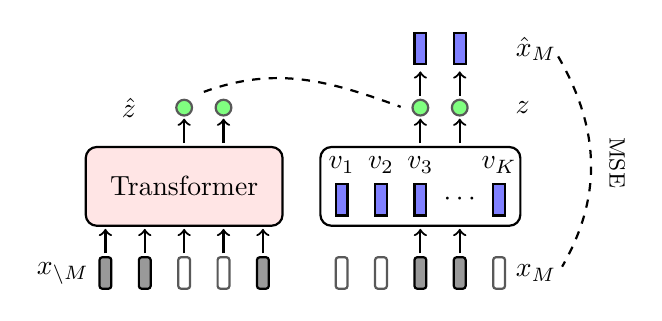
\begin{tikzpicture}[code/.style={draw, rectangle, fill=blue!50, inner sep=0.05cm, 
                                        minimum width=0.15cm, minimum height=0.4cm, thick}]

%
\node[code,rounded corners=1,fill=black!0,draw=black!65] (xb0) at (3.5, 0) {};
\node[code,rounded corners=1,fill=black!0,draw=black!65] (xb1) at (4, 0) {};
\node[code,rounded corners=1,fill=black!40] (xb2) at (4.5, 0) {};
\node[code,rounded corners=1,fill=black!40] (xb3) at (5, 0) {};
\node[code,rounded corners=1,fill=black!0,draw=black!65,label={right:$x_M$}] (xb4) at (5.5, 0) {};

%
%
%
%
\node[code,rounded corners=0] (xb2) at (4.5, 2.2+1.1-0.45) {};
\node[code,rounded corners=0] (xb3) at (5, 2.2+1.1-0.45) {};
\node[code,rounded corners=1,fill=black!0,draw=black!0,label={right:$\hat{x}_M$}] (xb4) at (5.5, 2.2+1.1-0.45) {};


%
\node[code,rounded corners=1,fill=black!40,label={left:$x_{\backslash M}$}] (xa0) at (0.5, 0) {};
\node[code,rounded corners=1,fill=black!40] (xa1) at (1, 0) {};
\node[code,rounded corners=1,fill=black!0,draw=black!65] (xa2) at (1.5, 0) {};
\node[code,rounded corners=1,fill=black!0,draw=black!65] (xa3) at (2, 0) {};
\node[code,rounded corners=1,fill=black!40] (xa4) at (2.5, 0) {};
\node [draw, rectangle, fill=red!10, thick, 
        rounded corners, minimum width=2.5cm, minimum height=1cm] (trans) at (1.5, 1.1) {Transformer};
%
\node[circle, thick, inner sep=0pt, minimum size=0.2cm, fill=green!50,draw=black!65] (za2) at (1.5, 2.1) {};
\node[circle, thick, inner sep=0pt, minimum size=0.2cm, fill=green!50,draw=black!65] (xa3) at (2, 2.1) {};
\node (z) at (0.8, 2.1) {$\hat{z}$};

%
\node[circle, thick, inner sep=0pt, minimum size=0.2cm, fill=green!50,draw=black!65] (xb2) at (4.5, 2.1) {};
\node[circle, thick, inner sep=0pt, minimum size=0.2cm, fill=green!50,draw=black!65] (xb3) at (5, 2.1) {};
\node (z) at (5.8, 2.1) {$z$};

%
\draw[->,thick] (0.5, 0.25) -- (0.5, 0.56);
\draw[->,thick] (1, 0.25) -- (1, 0.56);
\draw[->,thick] (1.5, 0.25) -- (1.5, 0.56);
\draw[->,thick] (2, 0.25) -- (2, 0.56);
\draw[->,thick] (2.5, 0.25) -- (2.5, 0.56);
%
\draw[->,thick] (2, 0.25+1.4) -- (2, 0.56+1.4);
\draw[->,thick] (1.5, 0.25+1.4) -- (1.5, 0.56+1.4);
%
\draw[->,thick] (4.5, 0.25+1.4) -- (4.5, 0.56+1.4);
\draw[->,thick] (5, 0.25+1.4) -- (5, 0.56+1.4);
%
\draw[->,thick] (4.5, 0.25+1.4+0.6) -- (4.5, 0.56+1.4+0.6);
\draw[->,thick] (5, 0.25+1.4+0.6) -- (5, 0.56+1.4+0.6);
%
\draw[->,thick] (4.5, 0.25) -- (4.5, 0.56);
\draw[->,thick] (5, 0.25) -- (5, 0.56);

%
%
\draw[dashed, thick] (1.75, 2.3) to [out=20, in=160] node[above] {\small $\KL$} (4.25, 0.56+1.55);
\draw[dashed, thick] (6.25, 2.2+1.1-0.55) to [out=-60, in=60] node[right, rotate=-90] {} (6.3, 0.08); 
\node[rotate=-90] (mse) at (7, 1.4) {\footnotesize MSE};

%
\node[code, label={above:$v_1$}] (v1) at (3.5, 0.93) {};
\node[code, label={above:$v_2$}] (v2) at (4, 0.93) {};
\node[code, label={above:$v_3$}] (v3) at (4.5, 0.93) {};
\node (v4) at (5, 0.93) {$\cdots$};
\node[code, label={above:$v_K$}] (v5) at (5.5, 0.93) {};
\draw[rounded corners, thick] (4.5-1.27, 0.6) rectangle (4.5+1.27, 1.6);
\end{tikzpicture}
\caption{HuBERT as variational predictive coding.
  The set $v_1, \dots, v_K$ are the codewords in the codebook,
  $x_{\backslash M}$ are the unmasked frames,
  and $x_M$ are the masked frames.
  There are two loss functions involved, the Kullback-Leibler divergence ($\KL$)
  and the mean-squared error (MSE).}
\label{fig:feedforward}
\end{figure}

\subsection{Quantization and Reconstruction}

%
In HuBERT, cluster IDs of frames that later serve as targets
for prediction are produced by $k$-means.
The $k$-means algorithm finds the ID of the closest centroid
for each individual frame, where closeness is defined by the $\ell_2$ loss.
To realize the quantization with $k$-means in our predictive coding framework,
we assign a point mass to the minimum and let
\begin{align}
q(z_i|x_i) = \mathbb{1}_{z_i = \argmin_{k=1, \dots, K} \|x_i - v_k\|^2},
\label{eq:argmin}
\end{align}
where $v_k$ is the $k$-th column of a matrix $V$, a codebook consisting of the centroids as columns.
Note that $q$ in principle can depend on $x_M$, but for this particular choice,
$q$ only depends on $x_i$.
%
%

The $k$-means objective is to minimize the distortion (or reconstruction) measured by the $\ell_2$ loss.
Given the codebook~$V$, using the cluster $z_i$ to reconstruct $x_i$ with the centroid $v_{z_i}$ gives a distortion $\|x_i - v_{z_i}\|^2$.
Naturally, we choose to parameterize $p(x_i|z_i)$ with a Gaussian and let
\begin{align}
p(x_i|z_i) = \frac{1}{(2\pi)^{d/2}}\exp\left(-\frac{1}{2}\|x_{i} - v_{z_{i}}\|^2\right),
\label{eq:rec}
\end{align}
where $d$ is the dimension of an acoustic frame.
The log of $p(x_i | z_i)$ gives the $\ell_2$ loss, i.e., the mean-squared error (MSE).
It is now clear that the term $\mathbb{E}_{z_i \sim q}[-\log p(x_i | z_i)]$ in equation \ref{eq:vlb-mlm} involves both the quantization of a frame $x_i$ and reconstructing it with the closest centroid $v_{z_i}$.
The negative entropy term $\mathbb{E}_{z_i \sim q}[\log q(z_i|x_i)]$ becomes 0 due to $q$ being a point mass.

\subsection{Predicting Quantized Frames}

Because $z_1, \dots, z_T$ correspond to the targets for prediction, we parameterize $p(z_i|x_{\setminus M})$
as a softmax, i.e.,
\begin{align}
p(z_i|x_{\setminus M}) = 
  \frac{\exp\left(\mathrm{enc}(x_{\setminus M})_i^\top u_{z_{i}}\right)}
    {\sum_{k=1}^K \exp\left(\mathrm{enc}(x_{\setminus M})_i^\top u_k\right)},
\label{eq:prior}
\end{align}
where $\mathrm{enc}(\cdot)$ is an encoder (typically a Transformer encoder),
%
$\mathrm{enc}(x_{\setminus M})_i$ is the $i$-th frame of the encoder output after taking the unmasked frames $x_{\setminus M}$ as input, and $u_k$ is the $k$-th column of the final linear layer~$U$.
The choice of $q(z_i|x_i)$ paired with the $p(z_i | x_{\setminus M})$ above completes the cross entropy $\mathbb{E}_{z_i \sim q}[-\log p(z_i | x_{\setminus M})]$ in equation~\ref{eq:vlb-mlm} for predicting the cluster IDs of frames.

\subsection{Two-Step Optimization}
\label{sec:optimization}

We have now instantiated the HuBERT objective from predictive coding.
The cross entropy term $\mathbb{E}_{z_i \sim q}[-\log p(z_i | x_{\setminus M})]$ and the reconstruction term $\mathbb{E}_{z_i \sim q}[-\log p(x_i | z_i)]$ are both present in the objective (equation \ref{eq:vlb-mlm}).
In principle, both terms should be optimized together,
but HuBERT takes a two-step approach, first finding the codebook by optimizing
the reconstruction (running $k$-means)
and then finding the Transformer parameters by optimizing the cross entropy.
The two-step approach is reminiscent to the variational view of expectation maximization \citep{neal1998view,attias1999variational}.
However, the codebook in HuBERT is never updated again after the first $k$-means,
and is said to be optimized offline as opposed to jointly with the Transformer
parameters.
This provides an opportunity to improve the optimization of the HuBERT objective.

\section{Extensions}
\label{sec:extensions}

%
Given how HuBERT is a special case of predictive coding, in this section, we discuss several immediate extensions that are made possible by our framework.

\subsection{Softening the Point Mass}

Even though the two-step optimization in HuBERT likely leads to suboptimal solutions, it turns out to be difficult to optimize both the cross entropy and the reconstruction together.
The difficulty stems from $q$ being a point mass, which cannot be optimized with gradient descent.
Instead of exact minimization, we can use soft-min and let
\begin{align}
q(z_i|x_i) = \frac{\exp\left(-\|x_i - v_{z_i}\|^2 / \tau\right)}
  {\sum_{k=1}^{K} \exp\left(-\|x_i - v_k\|^2 / \tau\right)},
  \label{eq:softmax-q}
\end{align}
where $\tau$ is the temperature.
As $\tau \to 0$, the distribution collapses to minimization or a hard $k$-means assignment \citep{Kulis2011RevisitingKN}, where each $x_i$ is assigned to the code $v_{z_i}$ with the smallest squared Euclidean distance.
With this parameterization, it is now possible to optimize the entire objective in equation \ref{eq:vlb-mlm} with gradient descent.
%

Since $q$ is no longer a point mass, we now have an additional negative entropy term $\mathbb{E}_{z_i \sim q}[\log q(z_i | x_i)]$ to optimize in equation \ref{eq:vlb-mlm}.
As entropy is maximized when $q$ is uniform, this term, when being minimized with other terms, encourages a diverse set of codes to be used and serves as a regularizer.
This is reminiscent to the diversity loss in wav2vec 2.0, and we will discuss the differences in later sections.

\subsection{Approximating the Expectation with Sampling}

Since $p(x_i | z_i)$ is parameterized in a relatively simple form, computing the expectation $\mathbb{E}_{z_i \sim q}[-\log p(x_i | z_i)]$ by enumerating all values of $z_i$, i.e., exact marginalization, is feasible.
However, exact marginalization is not always feasible when $p(x_i | z_i)$ becomes expensive to compute.
An alternative is to approximate the expectation with sampling.
There are various approaches to optimizing a function that involves sampling, and the simplest solution is to use Gumbel softmax \citep{jang2016categorical}.
We will compare marginalization and Gumbel softmax in the experiments.
Note that, the expectation is optimized offline with $k$-means in HuBERT, which will also be included in the comparisons.

\subsection{Future Prediction}
\label{sec:futurepred}

Our framework of predictive coding can also instantiate future prediction given the past.\footnote{Next-token prediction in language modeling, e.g., is a form of future prediction.}
The partition of a signal is a simpler than the masked prediction in that choosing a time point partitions the signal into the past and the future.
Formally, let $\mathcal{M}(x)$ be the stochastic process of choosing a time point $t$ in a signal $x$.
The past $x_{< t}$ and the future $x_{\geq t}$ forms a partition of $x$, and our autoregressive objective becomes
\begin{align}
\mathcal{L}_{\text{Future}} = \mathbb{E}_{(x_{< t}, x_{\geq t}) \sim \mathcal{M}(x)} [\mathcal{L}_{x_{< t}, x_{\geq t}}]
\end{align}
where
\begin{align}
\mathcal{L}_{x_{< t}, x_{\geq t}}
  = \sum_{i = t}^{T} & \mathbb{E}_{z_i \sim q} \big[ \log q(z_i|x_i) \label{eq:vlb-ar} \\
  & - \log p(z_i|x_{< i}) - \log p(x_i | z_i)]\big]. \notag
\end{align}
The form of equation \ref{eq:vlb-ar} is nearly identical to masked prediction in equation \ref{eq:vlb-mlm}, except the term $p(z_i | x_{< i})$.\footnote{The derivation of future prediction can be found in Appendix \ref{appendix:proof}.}
In terms of parameterization, $p(z_i | x_{< i})$ is typically modeled with a unidirectional LSTM or a causal Transformer; the rest of the terms remain the same.
Note that only the suffix of a signal participates in the objective, and $\mathcal{M}$ needs to be carefully chosen to avoid putting too much weight on the suffixes.
In practice, instead of choosing a time point at random, all frames are predicted with an equal amount of times \citep{oord2018representation,chung2019unsupervised}.

Since speech is generally smooth in time, an additional assumption $z_i \ind x_{i-\kappa+1:i} \mid x_{\leq i-\kappa}$ is commonly made for a small $\kappa > 0$ (e.g., in \citet{oord2018representation} and \citet{chung2019unsupervised}).
In other words, once we know the past frames $x_{\leq i-\kappa}$
close enough to the current time point $i$,
knowing additional few frames $x_{i-\kappa+1:i}$
does not add much information to $z_i$. 
The term $p(z_i | x_{< i})$ becomes $p(z_i | x_{\leq i-\kappa})$ under this assumption.

%
%
%
%
%
%
%
%
%
%
%
%
%
%
%
%
%
%
%
%
%
%
%
%
%
%
%
%
%
%
%
%
%
%
%
%
%
%
%
%
%
%
%
%
%
%
%
%
%
%
%

